\chapter{Patched MPO-MPO Contractions}
\label{chap:MPOcontr}
MPO-MPO contractions are widely recognized as a critical computational bottleneck in tensor-network algorithms, appearing frequently in applications like real-time evolution \cite{Paeckel2019}, finite-temperature simulations \cite{Verstraete2004}, two-particle field theory calculations \cite{Rohshap2025} and standard ground-state DMRG computations \cite{Schollwock2011}. Even when employing optimal contraction strategies, the computational complexity typically scales unfavorably with increasing bond dimensions rapidly becoming the dominant cost for large-scale calculations \cite{Schollwock2011,Rohshap2025,Paeckel2019}.

(Q)TCI makes it possible to encode intricate functions in a highly compact tensor‐train form, greatly facilitating the numerical evaluation of otherwise challenging integrals \cite{Fernandez2022,Fernandez2024,Rohshap2025}.  
Besides the favourable complexity of the TCI algorithm itself, a tensor representation is especially beneficial for convolution–type integrals, e.g.\ $h(x,y)\;=\;\int_{0}^{1}\! \mathrm{d}t\,f(x,t)\,g(t,y),$
because the integral can be carried out by simply contracting the tensor trains of the two integrands.  The contraction yields a ready‐made, reusable tensor‐train representation of the result~\(h\) employing MPO-MPO contraction routines.

While (Q)TCI substantially mitigates the cost of setting up convolution–type integrals, the subsequent MPO–MPO contraction still scales steeply with the bond dimensions of the two factors—typically $\order(\chi^{3}\kappa)$ or $\order(\chi^{2}\kappa^{2})$ \cite{Stoudenmire2010} , depending on the algorithm employed.  This rank dependence motivates \emph{distributing} the contraction across smaller sub-problems whose bond dimensions are capped, in the spirit of
patched QTCI.  We refer to such strategies collectively as \emph{patched MPO–MPO contractions}.

The remainder of this chapter is organised as follows: \prettyref{sec:MPOMPOcontr} reviews conventional MPO–MPO contraction schemes and establishes the notation used later;  \prettyref{sec:PatchMPOMPOContr} introduces the patched approach, analysing its advantages and resource scaling for several representative tensor products; finally,\prettyref{sec:AdaptivePatchMPOMPOContr} presents a new \emph{adaptive} contraction algorithm that, analogously to pQTCI, dynamically partitions the tensors and caps the local bond dimension, thereby balancing the contraction workload across patches.

\section{MPO-MPO Contractions: standard algorithms}
\label{sec:MPOMPOcontr}
A variety of well–established algorithms can contract two MPOs with high efficiency.  
Before reviewing these methods, we introduce the notation and conventions commonly adopted in the tensor-network literature, beginning with the central object of interest: the \textit{Matrix Product Operator} (\textit{MPO}).
\subsection{Matrix Product Operators}
Consider the tensor-train representation
\begin{equation}
    \widetilde{M}_{\bsigma\bsigma'} = \raisebox{-5.5mm}{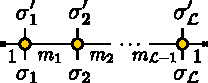
\includegraphics{figures/GenericMPO.pdf}}, \quad \text{with} \quad  M_\ell = \raisebox{-5.5mm}{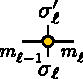
\includegraphics{figures/MPOSiteTensor.pdf}}.
\end{equation}
In the quantum-many-body community such a tensor train  with two physical legs per site is known as a \textit{Matrix Product Operator} (\textit{MPO}) \cite{Hubig2017, McCulloch2008, vonDelftTNNotes, Schollwock2011}. In numerical mathematics the same object appears under the name tensor-train operator (TTO) \cite{Oseledets2011}. Each four-legged core $M_\ell$ carries two virtual indices and two physical indices, and the largest virtual dimension $\chi = \max_\ell m_\ell$ is also called the rank of the MPO, mirroring the definition for matrix-product states (MPSs). MMPOs are routinely built to encode operators—Hamiltonians, density matrices, transfer matrices, projectors—that act on an MPS \cite{Hubig2017, Verstraete2008}. They underpin modern DMRG algorithms, time-evolution schemes, finite-temperature purification, and many other tensor-network techniques. 

The emergence of cross–approximation techniques has extended the relevance of MPOs to high–dimensional quadrature and convolution problems. A key property is that \emph{any} matrix-product state (MPS) can be recast as an MPO simply by fusing pairs (or groups) of physical indices. For an MPS comprising \(2\mathcal{L}\)
sites, the transformation is schematically
\begin{equation}
    \raisebox{-1.5cm}{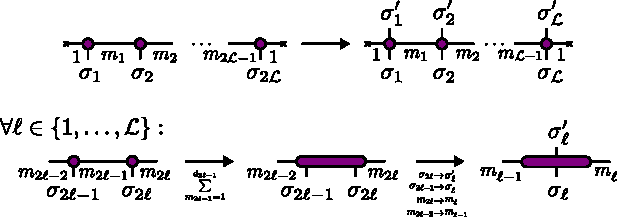
\includegraphics{figures/MPStoMPO.pdf}}
    \label{eq:MPStoMPO}
\end{equation}
where consecutive physical indices \((\sigma_{2\ell-1},\sigma_{2\ell})\) are merged into a single input–output pair
\(\bigl(\sigma_{2\ell-1},\sigma_{2\ell}\bigr)\equiv
 (\sigma'_{\ell},\sigma_{\ell})\).
This simple regrouping turns the state into an operator, enabling the same compressed representation to serve both as a multidimensional function and as an MPO contraction kernel.
For a generic MPS, one simply fuses multiple neighbouring indices—for example $\sigma_\ell,\sigma_{\ell+1},\sigma_{\ell+2} \to  (\sigma_\ell,\sigma_{\ell+1}),\sigma_{\ell+2}:=\sigma_\ell,\sigma'_\ell$—to obtain the desired operator form.

Given two matrix-product operators (MPOs)
\begin{equation}
    \widetilde{A}_{\bsigma'\bsigma''} = \raisebox{-7mm}{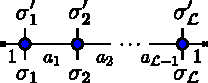
\includegraphics{figures/AMPO.pdf}}, \qquad \widetilde{B}_{\bsigma\bsigma'} = \raisebox{-5.5mm}{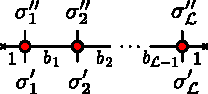
\includegraphics{figures/BMPO.pdf}}
    \label{eq:2MPOs}
\end{equation}
our goal is to form their product
\begin{equation}
    \raisebox{-8mm}{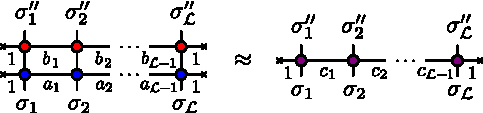
\includegraphics{figures/MPOMPOcontr.pdf}} := \widetilde{C}_{\bsigma\bsigma''}
\end{equation}

with tensor cores $C_\ell$. If $\widetilde{A}$ and $\widetilde{B}$ both have rank $\chi$ we want the final result $\widetilde{C}$ also to have rank $\simeq \chi$. Several contraction strategies exist. Below we outline the familiar \textit{zip-up} algorithm for completeness of this manuscript; alternative schemes available in modern tensor-network toolkits include the \textit{fitting} routine of Stoudenmire and White \cite{Stoudenmire2010} and the \textit{density-matrix} algorithm described in the tensornetwork.org documentation \cite{tensornetwork.org}.
\subsection{The zip-up algorithm}
Condider two MPOs of the form in \prettyref{eq:2MPOs}. For simplicity we will assume both to have rank $\chi$. The algorithm below illustrates how to efficiently contract them using the \textit{zip-up} method. 
\begin{figure}[ht!]
    \centering
    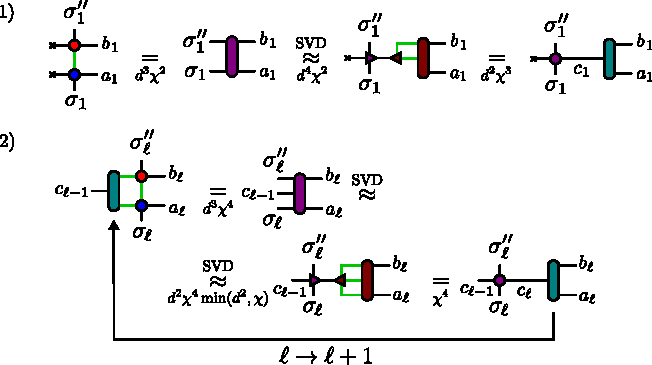
\includegraphics{figures/ZipUp.pdf}
    \caption{The zip-up MPO-MPO contraction algorithm. $(1)$ Start from the left-most site tensor contract the common physical index $\sigma'_1$. Decompose through SVD the four legged tensor, result of the first contraction by considering $(\sigma_1,\sigma''_1)$ and $(a_1,b_1)$ the row column index of the matrix. The left isometry, \raisebox{-0.1mm}{
\includegraphics{figures/LeftIsometry.pdf}} out of SVD will be the new core of the MPO product. The decomposition will be truncated either by fixing the maximal rank of of \raisebox{-0.1mm}{
\includegraphics{figures/LeftIsometry.pdf}} (as a matrix) or by setting a local cutoff for the singular values $\varepsilon_{\text{loc}}$. Contract the remaining matrices of the SVD decomposition into a single tensor and proceeds to the next site. $(2)$ }
\end{figure}


\section{Patched MPO-MPO Contractions }
\label{sec:PatchMPOMPOContr}
\subsection{Patched contraction logic}
The output produced by pQTCI contains objects with the schematic form

\begin{equation}
    \raisebox{-7mm}{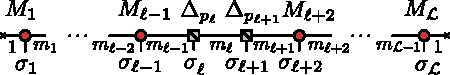
\includegraphics{figures/MultplePatchMPS.pdf}}.
    \label{eq:patchedMPS}
\end{equation}

Suppose we promote this patched MPS to an MPO so that it can enter subsequent contractions.  The local mapping depends on the site index~$\ell$, hence on the way the MPO is folded; from \prettyref{eq:MPStoMPO} one obtains
\begin{align}
    \label{eq:patchMPStoMPO}
        \nonumber &\raisebox{-0.6cm}{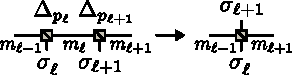
\includegraphics{figures/patchMPStopatchMPO_SiteTensor.pdf}} &=&\quad \begin{cases}
		[\mathds{1}]_{m_{\ell-1},m_{\ell+1}} & \text{if } \sigma_\ell = p_\ell \wedge \sigma_{\ell +1} = p_{\ell +1}\\
		0 & \text{otherwise},
        \end{cases}\\[6pt]
        &\raisebox{-0.6cm}{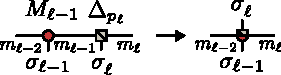
\includegraphics{figures/patchMPStoBottomHalfPatchMPO.pdf}} &=&\quad \begin{cases}
		[M^{\sigma_{\ell-1}}]_{m_{\ell-2},m_{\ell}} & \text{if }\sigma_\ell = p_\ell\\
		0 & \text{otherwise},
        \end{cases}\\[6pt]
        \nonumber &\raisebox{-0.6cm}{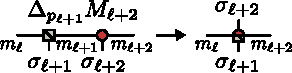
\includegraphics{figures/patchMPStoTopHalfPatchMPO.pdf}} &=& \quad \begin{cases}
		[M^{\sigma_{\ell+2}}]_{m_{\ell},m_{\ell+2}} & \text{if } \sigma_{\ell+1} = p_{\ell+1} \\
		0 & \text{otherwise}.
        \end{cases}  
\end{align}

Hence, when contracting two patched MPOs of the type in \prettyref{eq:patchedMPS}, the product is
non--vanishing only if the projected indices coincide on \emph{all} internal legs.  Consider, for example, the two MPOs
\begin{equation}
    \label{eq:patchMPOs}
    \begin{aligned}
        \widetilde{A}^{p''_3,p''_4}_{\bsigma'\bsigma''} &= \raisebox{-7mm}{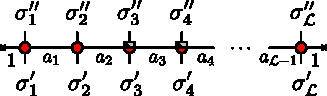
\includegraphics{figures/AProjMPO.pdf}} \\ 
        \widetilde{B}^{p_2,p'_2,p_3,p'_4}_{\bsigma\bsigma'} &= \raisebox{-5.5mm}{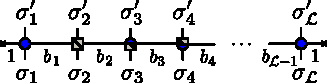
\includegraphics{figures/BProjMPO.pdf}}.
    \end{aligned}  
\end{equation}
They always yield a result of the form

\begin{equation}
    \label{eq:resultPatchContr}
        \widetilde{C}^{p_2,p_3,p''_3,p''_4}_{\bsigma\bsigma''} = \raisebox{-7mm}{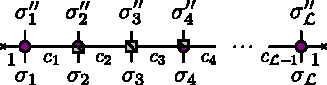
\includegraphics{figures/CProjMPO.pdf}}.
\end{equation}

By contrast, two MPOs shaped as
\begin{equation}
    \label{eq:patchMPOsMaybe}
    \begin{aligned}
        \widetilde{A}^{p'_2,p'_3,p''_3}_{\bsigma'\bsigma''} &= \raisebox{-7mm}{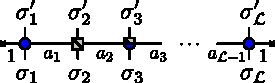
\includegraphics{figures/AProjMPO_vanish.pdf}} \\ 
        \widetilde{B}^{p_2,p'_2,p'_3}_{\bsigma\bsigma'} &= \raisebox{-5.5mm}{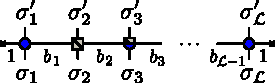
\includegraphics{figures/BProjMPO_vanish.pdf}}
    \end{aligned}  
\end{equation}

produce a non--zero contraction only when the projected internal indices match, \textit{i.e.} $p'^{A}_{2}=p'^{B}_{2}$ and $p'^{A}_{3}=p'^{B}_{3}$.  In other words, to obtain a non--vanishing outcome, any internal index that is projected must be projected onto the \emph{same} value in both factors; the external indices place no such restriction. 

Assume that two tensors \(A_{\boldsymbol{\sigma}}\) and
\(B_{\boldsymbol{\sigma}}\) have been decomposed by pQTCI into collections of
patches,
\begin{equation}
    \label{eq:patchCollectionsContr}
  A_{\bsigma}
    \;\approx\;
    \sum_{\widetilde{A}^{(i)}\in\texttt{results}_{A}}\,
        \widetilde{A}^{(i)},
  \qquad
  B_{\boldsymbol{\sigma}}
    \;\approx\;
    \sum_{\widetilde{B}^{(j)}\in\texttt{results}_{B}}\,
        \widetilde{B}^{(j)}.
\end{equation}
After promoting each patch to MPO form, the full contraction
\(C_{\bsigma}\) can be assembled patch-wise:
contract every patch \(\widetilde{A}^{(i)}\) with each \emph{compatible} patch \(\widetilde{B}^{(j)}\) (i.e.\ those whose projected internal indices match).  This yields a family of subtensors \(\{\widetilde{C}^{(k)}\}\) which, upon MPO-to-MPS unfolding (cf.\ \prettyref{eq:resultMPSPatchContr}),collectively approximate the target tensor \(C_{\bsigma}\). In other words each TT of $\texttt{results}_{A}$ will be contracted with every TT in $\texttt{results}_{B}$ and depending on the compatibility of the projection (cf. \prettyref{eq:patchMPOsMaybe}) result in a TT $\widetilde{C}^{(k)}$ part of the patched representation of \(C_{\bsigma}\). The subsequent section will help us clarify this concept with a graphical representation of the \textit{patched contraction}.

\subsection{Patch contraction 2D representation}
The product MPO in \prettyref{eq:resultPatchContr} can be unfolded back into a patched MPS by inverting the mapping of \prettyref{eq:MPStoMPO}. To do so, one may perform an SVD or a CI/prrLU on each MPO site tensor or simply read off the local cores from \prettyref{eq:patchMPStoMPO}. The resulting MPS reads
\begin{align}
    \label{eq:resultMPSPatchContr}
     \nonumber \widetilde{C}^{p_2,p_3,p''_3,p''_4}_{\bsigma} &= \raisebox{-6mm}{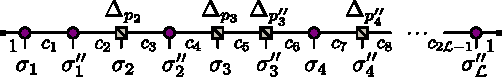
\includegraphics{figures/PatchMPS_ResultContr.pdf}}\\
     {}\\[-5pt]
    \nonumber \widetilde{C}^{p_3,p_5,p_6,p_8}_{\bsigma} &= \raisebox{-6mm}{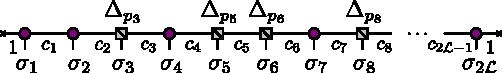
\includegraphics{figures/PatchMPS_ResultContrReshaped.pdf}}
\end{align}
where the second equality is obtained after relabelling site indices and bond dimensions.
The auxiliary cores $\Delta{p_{\ell}}$ encode the subtensor corresponding to the external (non--contracted) indices of $\widetilde{A}$ and $\widetilde{B}$, \textit{i.e.} external projected indices in $\widetilde{A}$ and $\widetilde{B}$ will be projected indices in $\widetilde{C}$. Moreover, each physical index and each core $A_{\ell}$, $B_{\ell}$ in the original MPS factors may be a composite of neighbouring indices and cores, rendering the resulting sitensors $C_{\ell}$ and assigned indices also a composition of neighbouring sites. 

The tensor‐train in \prettyref{eq:resultMPSPatchContr} closely mirrors the TT form of an individual patch produced by the pQTCI algorithm. If each TT physical index has dimension $d_\ell = 2$ we can assume to be working with a two–dimensional, interleaved quantics representation and each such MPS corresponds to a distinct sub-region of the 2D domain, uniquely labelled by its prefix indices. A full set of these patches can tile the entire domain; when their contributions are summed, they collectively furnish a single TT approximation of an underlying tensor. 

This insight suggests a convenient two-dimensional diagrammatic view of patched contractions. Let us introduce three quantics variables on the unit interval, each resolved with $\mR$ binary digits,
\begin{equation}
    \begin{gathered}
        x \to x(\bsigma) = \sum_{r=1}^{\mR} \sigma_r 2^{-r} \quad y \to y(\bsigma') = \sum_{r=1}^{\mR} \sigma'_r 2^{-r}\\ 
        s \to s(\bsigma'') = \sum_{r=1}^{\mR} \sigma''_r 2^{-r}.
    \end{gathered}
\end{equation}
With this notation, the patch ensembles introduced in \prettyref{eq:patchCollectionsContr}—and the tensor that results from their pairwise contractions—can be depicted in the following schematic.

\begin{figure}[ht!]
    \centering
    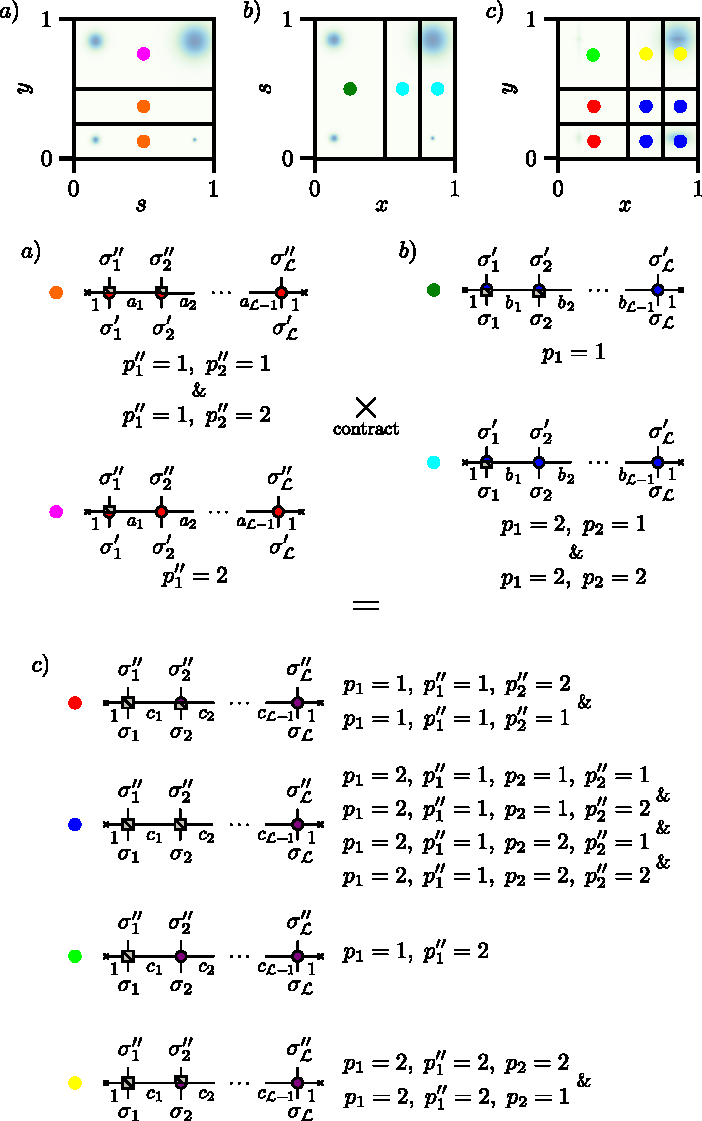
\includegraphics{figures/2DPatchContrRepr.pdf}
    \caption{2D Patch Contraction}
\end{figure}

\subsection{Patched Element-wise Multiplication}
Let $\widetilde{A}_{\bsigma}$ and $\widetilde{B}_{\bsigma}$ be two MPSs.  We seek their \textit{Hadamard (element-wise) product} \cite{Lee2018}
\begin{equation}
    C_{\bsigma} = A_{\bsigma}\,\raisebox{.5pt}{\textcircled{\raisebox{-3pt}{*}}}\,B_{\bsigma}
\end{equation}
meaning that every entry of $C$ is obtained by multiplying the corresponding entries of $A$ and $B$; $C_{\bsigma} = A_{\bsigma}B_{\bsigma}$ for all index tuples $\bsigma$. 
To carry out the element-wise product we first embed each tensor train in a \emph{diagonal} MPO:
\begin{equation}
    \begin{aligned}
       \widetilde{A}_{\bsigma} &= \raisebox{-7mm}{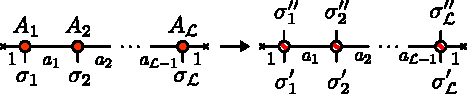
\includegraphics{figures/ADiagMPO.pdf}} := \widetilde{A}^D_{\bsigma'\bsigma''}\\
       \widetilde{B}_{\bsigma} &= \raisebox{-7mm}{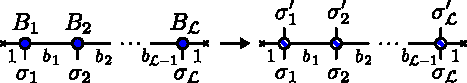
\includegraphics{figures/BDiagMPO.pdf}} := \widetilde{B}^D_{\bsigma\bsigma'}
    \end{aligned}
    \label{eq:diagMPOs}
\end{equation}

where each local tensor is defined by

\begin{equation}
    \begin{aligned}
        \raisebox{-6mm}{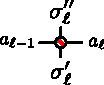
\includegraphics{figures/ADiag_SiteTensor.pdf}} = \begin{cases}
            [A^{\sigma'_\ell}_\ell]_{a_{\ell-1},a_\ell} \quad &\text{if}\ \sigma'_\ell = \sigma''_\ell \\
            [0]_{a_{\ell-1},a_\ell} \quad &\text{otherwise}
        \end{cases}\\
        \raisebox{-6mm}{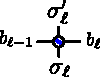
\includegraphics{figures/BDiag_SiteTensor.pdf}} = \begin{cases}
            [B^{\sigma_\ell}_\ell]_{b_{\ell-1},b_\ell} \quad &\text{if}\ \sigma_\ell = \sigma'_\ell \\
            [0]_{b_{\ell-1},b_\ell} \quad &\text{otherwise}
        \end{cases}
    \end{aligned}
\end{equation}
and $0_{m,n}$ denotes the element $(m,n)$ of the zero matrix.
The site indices of the original TTs have been relabelled to make the subsequent contraction explicit:
\begin{equation}
    \raisebox{-0.8cm}{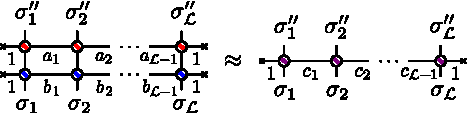
\includegraphics{figures/DiagMPOMPOcontr.pdf}}.
    \label{eq:diagMPOcontr}
\end{equation}
From this contraction we read off the resulting tensor-train
\begin{equation}
    \widetilde{C}_{\sigma} = \raisebox{-5.5mm}{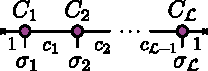
\includegraphics{figures/CTensorTrain.pdf}} \quad \text{with} \quad \raisebox{-6.5mm}{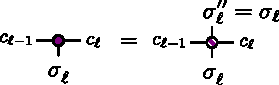
\includegraphics{figures/UnDiag_SiteTensor.pdf}}.
\end{equation}
Hence $\widetilde{C}$ represents the Hadamard product
$C_{\boldsymbol{\sigma}}=A_{\boldsymbol{\sigma}}B_{\boldsymbol{\sigma}}$ in TT form. The MPO-MPO contraction in \prettyref{eq:diagMPOcontr} can be performed using the standard Tensor Network toolkit, however in the case where we performed the patching routine upon the tensors 


\begin{figure}[ht!]
    \caption{Heatmap + patch grid of element-wise multiplication of 2D MPOs (qHO calculation of $\Psi^2(x)$ ) }
\end{figure}

\todo{Benchmark with Quantum Harmonic Oscillator in localised potential ($\omega \gg 1$) $\to$ evaluate $|\Psi(x)|^2$. Also something related to heat equation could work}

\begin{figure}[ht!]
    \caption{Number of patches vs patch bond dimension with optimal region for element-wise multiplication ( theoretical value) }
\end{figure}

\begin{figure}[ht!]
    \caption{Memory and time scaling element-wise multiplication + fit  }
\end{figure}
\subsection{Patched Matrix Multiplication}

Let \(\widetilde{L}_{\boldsymbol{\sigma}}\) and \(\widetilde{R}_{\boldsymbol{\sigma}}\) be two generic matrix-product states (MPS).  The first carries index sets \(\boldsymbol{\sigma}^{R},\boldsymbol{\sigma}^{S}\), the second \(\boldsymbol{\sigma}^{S},\boldsymbol{\sigma}^{C}\).  
Using the mapping of Eq.~\eqref{eq:MPStoMPO}, each MPS can be reshaped into an MPO:
\begin{align}
       \nonumber\widetilde{L}_{\bsigma} &= \raisebox{-7mm}{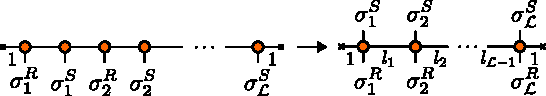
\includegraphics{figures/LeftMPO.pdf}} := \widetilde{L}_{\bsigma^R\bsigma^S}\\
       {}\\
        \nonumber\widetilde{R}_{\bsigma} &= \raisebox{-7mm}{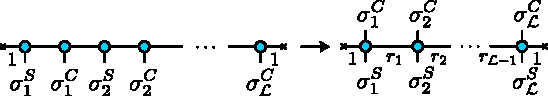
\includegraphics{figures/RightMPO.pdf}} := \widetilde{R}_{\bsigma^S\bsigma^C}
    \end{align}
    \label{eq:matMulMPOs}


Here each composite index (e.g.\ \(\sigma^{R}_{\ell}\)) can represent a single index or a a block of neighbouring
physical indices of a parent MPS and every MPS core is obtained by contracting the corresponding block of neighbouring MPS tensors.

With this interpretation, the contraction
\begin{equation}
    \widetilde{M}_{\bsigma^R\bsigma^C} = \sum_{\bsigma^S} \widetilde{L}_{\bsigma^R\bsigma^S}\widetilde{R}_{\bsigma^S\bsigma^C} = \raisebox{-10mm}{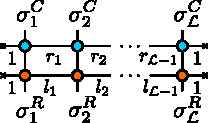
\includegraphics{figures/MatMulMPOContr.pdf}}
\end{equation}

acts exactly like a \emph{matrix multiplication} between two tensor-train–style objects, producing an MPO indexed by
\(\boldsymbol{\sigma}^{R}\) and \(\boldsymbol{\sigma}^{C}\). The labeling becomes then much clearer: $\bsigma^R$, $\bsigma^C$ and $\bsigma^S$ represent the row, column and shared indices of our ``matrices'' $L$ and $R$.

\begin{figure}[ht!]
    \caption{Heatmap + patch grid of matrix multiplication of 2D MPOs with worst, average and best case scenario for patch subdivision (linear combination of gaussians). }
\end{figure}

\begin{figure}[ht!]
    \caption{Number of patches vs patch bond dimension with optimal region for matrix multiplication (theoretical value) }
\end{figure}

\begin{figure}[ht!]
    \caption{Memory and time scaling matrix multiplication + fit  }
\end{figure}


\section{Adaptive Patched MPO-MPO Contraction}
\label{sec:AdaptivePatchMPOMPOContr}

\begin{figure}[ht!]
    \centering
    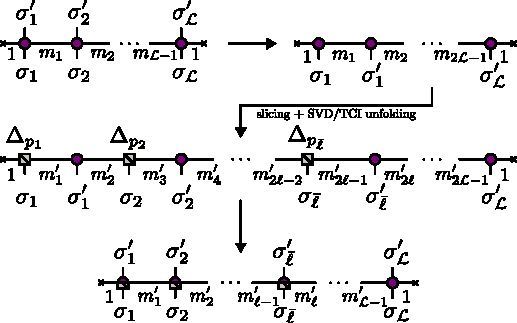
\includegraphics{figures/SlicingMPO.pdf}
    \caption{Slicing of an MPO}
\end{figure}

\begin{figure}[ht!]
    \centering
    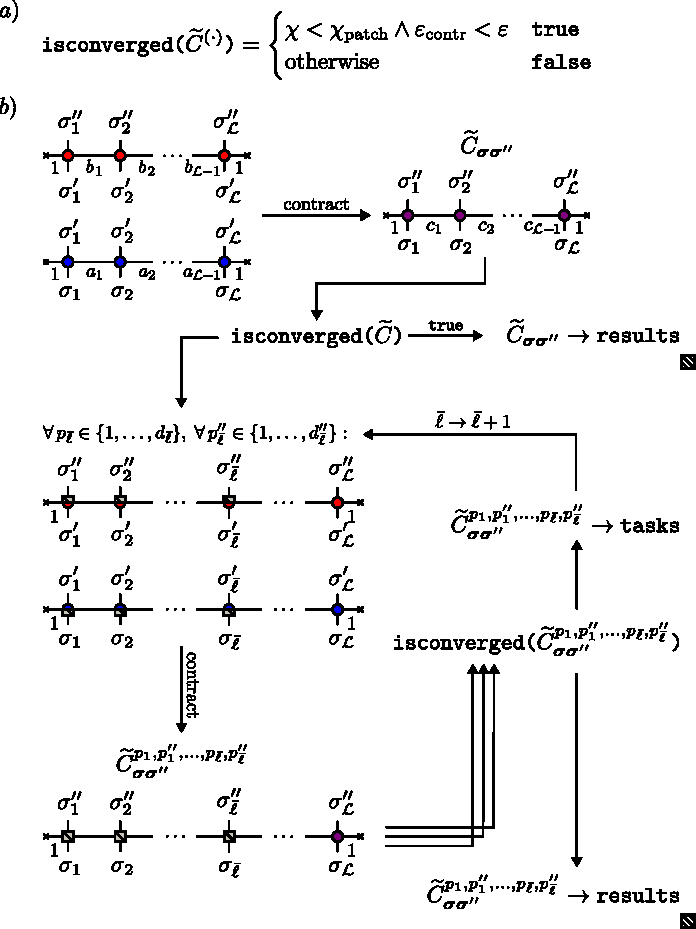
\includegraphics{figures/AdaptivePatchContr.pdf}
    \caption{Adaptive Patched Contraction }
\end{figure}

\begin{figure}[ht!]
    \caption{Heatmap + patch grid of adaptive matrix multiplication (linear combination of gaussians). }
\end{figure}

\begin{figure}[ht!]
    \caption{Memory scaling matrix multiplication compared with normal patch contraction }
\end{figure}


